% \mychapter{Final Considerations and Schedule}{cap:conclusion}
% \lhead{FINAL CONSIDERATIONS}

% This works' purpose is to improve the mobile experience in 5G networks through SDNs. We presented a mathematical model to allocate users of mobile networks in base stations. According to the model, handovers should happen considering the shortest distance between eNBs and UEs, handover average, base stations and the users bandwidth requirements, and also the signal strength between users and base stations. We achieve results for the model defined according to \eqref{equ:users} and \citet{tarik2015} optimizations for minimizing handover between coverage areas and the communication costs between eNBs and data centers.

% In the following steps, we will evaluate the improvement of the (COMP) model composed with Equation \eqref{equ:users2} and the heuristic solution. Also, we must simulate each model in a network environment, provided by simulators such as ns3, and evaluate the models against different mobility models.

% The proposal for a heuristic solution, which is based on an iterated local search combined with random variable neighborhood search, is motivated by the need for a sufficiently good solution, which can be used upon software or hardware computational restrictions. The search algorithms are complement by four neighborhood structures, which are swaps and insertion operations upon users and base stations. 

% When verified the correct functioning of the models, we will proceed to the implementation in network simulators that can support SDN applications. The execution of the models in simulators will allow us to observe the impact on factors such as transfer rates, load balancing, and mobility experience. The simulation will consider different mobility models, such as the random waypoint, random walk, random direction, street random waypoint, reference point group model (RPGM), Manhattan mobility, and freeway mobility.


% The execution of these activities will follow the working schedule presented in figure \ref{fig:schedule}, which are described below.

% \begin{figure}[h]
%     \centering
%     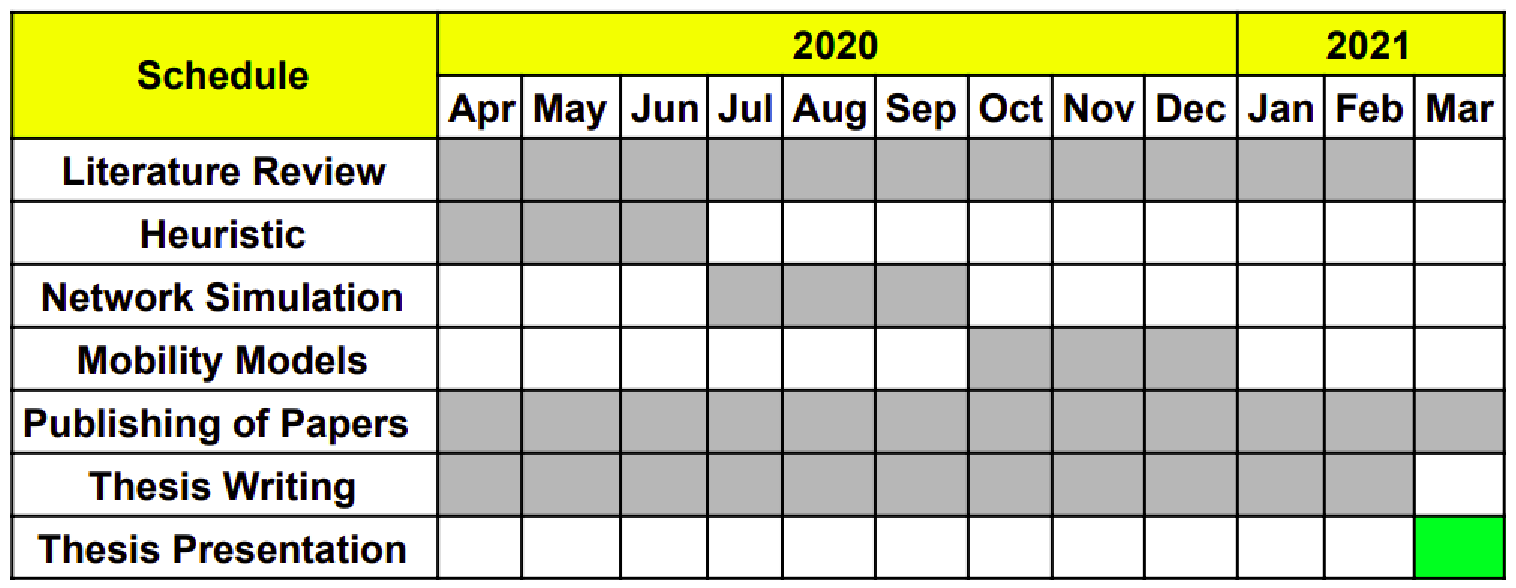
\includegraphics[width=.8\textwidth]{img/schedule.pdf}
%     \caption{Master's working schedule for 2020 and 2021.}
%     \label{fig:schedule}
% \end{figure}

% %% Alla - coloca todos esses itens detalhados e explicando aqui o que consiste cada uma dessas etapas.

% \begin{itemize}
%     \item {\bf Literature review:} This step consists of reviewing the relevant literature. The process is continuous and lasts practically throughout all the master's period. It is very important that our reading is up to date the current works and state-of-the-art techniques that can be applied;
%     \item {\bf Heuristic}: This step, which lasts for three months (from April to June), consists of the development and execution of heuristic methods (ILS + RVND). We will also look for alternative methods to the heuristic iterated local search;
%     \item {\bf Network simulation}: In the simulation step, lasting from July to September 2020, solutions will be implemented in network simulation environments that can support SDN applications. With the simulation results, it is expected to assess the impact of the models on transfer rates, network's load balance, and user connectivity;
%     \item {\bf Mobility models}: Between October and December, we have the phase of evaluating the behavior of the network and the proposed solutions according to mobility models, such as random waypoint, random walk, random direction, street random waypoint;
%     \item {\bf Publishing of papers}: The publishing of articles in the relevant scientific media, such as journals, congresses, and conferences, will last throughout all the development of this work, and will occur whenever any relevant results are discovered;
%     \item {\bf Thesis writing}: The writing of the thesis is incremental, and will take place for almost the entire duration of this work;
%     \item {\bf Thesis presentation}: To Consolidate the results and the written thesis, this work will be presented in March 2021.
% \end{itemize}

